%space 

\setlength{\textfloatsep}{0.45cm}
\setlength{\floatsep}{0.45cm}
\begin{algorithm}[t]
\caption{Safe RL with BRSL}
\label{alg:rlwithbrsl}
% \begin{algorithmic}[1]
\textbf{initialize} the RL agent with a random policy $\policy_\theta$, environment model $\mimic_\phi$, empty replay buffer $B$, max number of time steps $\niter$, and a safe plan $\plan_0$
% Collect $N_{\coef}$ $<_k, a_k, r_k, x(k + 1)>$

\For{each episode}{
    \textbf{initialize} task with reward function $\rewfunc$
    
    $\RLstate_1 \leftarrow $ observe initial environment state \label{ln:observe1}
    
    \For{$k = 1:\niter$}{
        
    %     $\plan_k \leftarrow \dreamfunc{\RLstate_k,\policy_\theta,\mimic_\phi}$ // use Alg. \ref{alg:dream} \label{ln:init_plan_by_dreaming}
    \tbold{ $\plan_k \leftarrow$ roll out a trajectory}
     
         $\reachapprox_k \leftarrow \zono{\vcstate_k,\zeros}$ // init. reachable set \label{ln:initZono}
        
         $\left(\reachapprox_j\right)_{j=k}^{k+\nplan} \leftarrow \reachfunc{\reachapprox_k,\plan_k}$ // use Alg. \ref{alg:LipReachability}  \label{ln:reachAlg1}
        
        \If{any $\reachapprox_j \cap \statespace\obs \neq \emptyset$ \label{ln:if_unsafe}}{
            
            \textbf{try} $\plan_k \leftarrow \adjustfunc{\plan_k,\statespace\obs}$ // use Alg. \ref{alg:adjust}
            
            \textbf{catch} execute failsafe maneuver; continue\label{ln:catch_unsafe} 
            %``unsafe'' $\plan_k \leftarrow \plan_{k-1}$ // keep old plan\label{ln:catch_unsafe}
        }
        
        $\action_k \leftarrow$
        get first (safe) action from $\plan_k$ \label{ln:get_safe_action}

         $r_k \leftarrow \rewfunc(\RLstate_k,\action_k)$ // get reward \label{ln:getReward}
        
         $\RLstate_{k + 1} \leftarrow $ observe next environment state \label{ln:observe2}
        
         \textbf{add} $(\RLstate_k, \action_k, r_k, \RLstate_{k + 1})$ to $B$ \label{ln:addToBuffer}
        
         \textbf{train} the RL agent $\policy_\theta$ and the environment model $\mu_\phi$ using minibatch from $B$ \label{ln:train_rl_agent}
    }
}
% \end{algorithmic}
\end{algorithm}

\section{Black-box Reachability-based Safety Layer}\label{sec:solu}

\tbold{We unite three components into our BRSL system for collision-free motion planning without a dynamic model of the robot or its surroundings \textit{a priori}.
The first component is an environment model, learned online.
To find high reward actions (i.e., motion plans) for this model, the second component is an RL agent.
Since the agent may create unsafe plans, our third component is a safety layer that combines data-driven reachability analysis with differentiable collision checking to enable safe trajectory optimization.
Theorem \ref{thm:BRSL_is_safe} summarizes safety via BRSL.}

% Our method, shown in Fig. \ref{fig:framework}, guarantees safety by preventing the RL agent from taking unsafe actions.
% When an agent chooses an unsafe plan, BRSL
% \begin{enumerate}[label=(\alph*)] %[leftmargin=15pt,noitemsep,partopsep=0pt,topsep=0pt,parsep=0pt]
% % \itemsep0em 
% \item prevents the execution of the unsafe plan,
% \item penalizes the agent with a negative reward, and 
% \item replaces the agent's plan with a safe and feasible plan.
% \end{enumerate}
% Note that the penalty helps the RL agent to learn avoiding choosing unsafe actions or frequently activating the safety layer since the safe replacement plan does not necessarily aid task completion. 
% The safety layer makes use of an existing method for data-driven reachability analysis of a black-box system \cite{alanwar2020data} as one component, which overapproximates a reachable set from noisy data under mild noise assumptions.





% \subsection{Algorithm Overview}
%textbf{Overview.}
BRSL is summarized in Algorithm \ref{alg:rlwithbrsl}.
It uses a receding-horizon strategy to create a new safe plan $\plan_k$ in each $k$\ts{th} receding-horizon motion planning iteration.
Consider a single planning iteration (that is, time step $k$) (Lines \ref{ln:observe1}--\ref{ln:train_rl_agent}).
Suppose the RL agent has previously created a safe plan $\plan_{k-1}$ (such as staying stopped indefinitely).
At the beginning of the iteration, BRSL creates a new plan $\plan_k$ by rolling out the RL agent along with an environment model. %; we call this process \emph{dreaming} (Line \ref{ln:init_plan_by_dreaming} and Algorithm \ref{alg:dream}).
Next, BRSL chooses a safe action by adjusting the \tbold{rolled-out} action sequence (Lines \ref{ln:if_unsafe}--\ref{ln:catch_unsafe}) such that the corresponding reachable set (computed with Algorithm \ref{alg:LipReachability}) is collision-free and ends with a failsafe maneuver. 
If the adjustment procedure (as in Algorithm \ref{alg:adjust}) fails to find a safe plan, then the robot executes the  failsafe maneuver.
Finally, BRSL sends the first action in the current safe plan to the robot, gets a reward, and trains the RL agent and environment model (Lines \ref{ln:get_safe_action}--\ref{ln:train_rl_agent}). 
To enable training our environment model online, we collect data in a replay buffer $B$ at each time $k$ (Line \ref{ln:addToBuffer}).
We note that BRSL can be used during both training and deployment.
That is, the safety layer can operate even for an untrained policy.
Thus, for training, we initialize $\policy_\theta$ with random weights.

\tbold{To proceed, we detail our methods for data-driven reachability and adjusting unsafe actions.}

%\begin{algorithm}[t]
\caption{Dreaming}
\label{alg:dream}
\KwInput{current RL agent state $\RLstate_k$, RL policy $\policy_\theta$, and environment mimic network $\mimic_\phi$}

\KwInOut{reward $\rewfunc$ and action $\action\brk$ per Assum. \ref{assumption:stop}}

$\dreamstate_k \leftarrow \RLstate_k$ // initialize dream state

\For{$j = k:(k+\nplan)$ \label{ln:dream1}}{
     $\mimicaction_j \leftarrow \policy_\theta(\dreamstate_j)$ // dream action \\ \label{ln:dream2}
     
     $\rew_j \leftarrow \rewfunc(\dreamstate_j,\mimicaction_j)$ // dream reward

     $\dreamstate_{j+1} \leftarrow \mimic_\phi(\dreamstate_{j+1},\mimicaction_j)$ // dream next state \\ \label{ln:dream3}
} \label{ln:dream4}

$\mimicaction_j \leftarrow \action\brk$ for all $j > k + \nplan$ // include failsafe \\

 \textbf{return} $\plan_k \leftarrow (\mimicaction_j)_{j=k}^\infty$ // dreamed plan
\end{algorithm}



%  \subsection{Dreaming}~
% %\textbf{Dreaming.}
% To ensure safety, BRSL must reason about the entire future trajectory of the robot, but cannot directly predict the future trajectory and observations since it does not have access to the environment model. 
% Instead, we let the agent \emph{dream} future environment states by training an \emph{environment mimic}, $\mimic_\phi: (\RLstate_k,\action_k) \mapsto \dreamstate_{k+1}$, where $\dreamstate_{k+1} \in \R^\nrl$ is the dream state, and $\phi$ are the network parameters.
% % We use the dreamed states to predict the future trajectory.
% We implement $\mimic_\phi$ as an ensemble of neural networks (see Section \ref{sec:eval}).
% Using the data $(\RLstate_k,\action_k,\rew_k,\RLstate_{k+1})$ in the replay buffer $B$, we train the mimic online to minimize expected mean squared error between $\RLstate_{k+1}$ and $\mimic_\phi(\RLstate_k,\action_k)$.

% Dreaming is summarized in Algorithm \ref{alg:dream}.
% At each time $k$, the mimic takes in the RL agent state and action and estimates the next RL agent state.
% Then, the dream state is given to the RL agent to predict an action $\action_{k+1} = \policy_\theta(\dreamstate_{k+1})$.
% This process is repeated $\nplan$ times.
% Since our goal is to ensure safety, the length $\nplan$ should be large enough that a failsafe maneuver is possible, meaning braking the robot to a stop per Assumption \ref{assumption:stop}; so, $\nplan$ must be greater than the number of time steps $n\brk$ required to stop from maximum speed \cite{kousik2020bridging}.
% Note, the failsafe maneuver can be more complex, such as moving an autonomous car off the road \cite{magdici2016fail} or through an intersection \cite{vaskov2019not}.





 \subsection{Data-Driven Reachability Analysis}\label{subsec:data_driven_reachability_analysis}
 
\begin{algorithm}[t]
\caption{Black-box System Reachability \cite{alanwar2020data_conf}}\label{alg:LipReachability}
\KwInput{initial reachable set $\hat{\reachset}_0$, actions $(\action_j)_{j=k}^{k+\nplan}$} %, time-varying action space $(\actionspace_k)_{k=0}^{n}$

\KwInOut{state/action data $\data$, noise zonotope $\noisespace = \zono{\ctr_\noise,\Gen_\noise}$, Lipschitz constant $L^\star$, covering radius $\delta$}
    
% $\reachapprox_{0} \leftarrow \statespace_0$ // init. reachable set

\tbold{
$Z_\epsilon \leftarrow \zono{\zeros,\diag{\arridx{\vc{L^\star}}{1} \arridx{\vc{\delta}}{1}/2,\cdots,\arridx{\vc{L^\star}}{n} \arridx{\vc{\delta}}{n}/2}}$ \label{ln:alglipZeps}
}
\For{$j = k:(k+\nplan)$}{      
    % $\vc{M}_j \leftarrow \left(\statedata_+ - [\ctr_\noise,\cdots,\ctr_\noise] \right)\begin{bmatrix} 
    % \ones_{1 \times t\total}\\ \statedata_--1 \otimes \vcstate^\star_j \\ \actiondata-1 \otimes\action_j
    % \end{bmatrix}^\dagger$ \label{ln:alglipMtilde}
    
    \tbold{$\vc{M}_j \leftarrow \left(\statedata_+ - \ctr_\noise\right)
        \begin{bmatrix} 
            \ones_{1 \times t\total} \\
            \statedata_- - \vcstate^\star_j \\
            \actiondata - \action_j
        \end{bmatrix}^\dagger$ \label{ln:alglipMtilde}}
    
    % $\lb  \leftarrow \min_j \Bigg( {(\statedata_{+})}_{:\,,j} - \vc{M}_j \begin{bmatrix} \ones \\
    % {(\statedata_-)}_{:\,,j} -  \vcstate^\star_j\\ {(\actiondata)}_{:\,,j} - \action_j \end{bmatrix} \Bigg)$
    
    $\lb  \leftarrow \min_j \Bigg( {(\statedata_{+})}_{:\,,j} - \vc{M}_j
        \begin{bmatrix}
            1 \\
            {(\statedata_-)}_{:\,,j} -  \vcstate^\star_j \\
            {(\actiondata)}_{:\,,j} - \action_j
    \end{bmatrix} \Bigg)$
    
    $\ub \leftarrow$ same as $\lb$, but use max instead of min  \label{ln:alglipupper}
    
    %$\ub \leftarrow$ same as $\lb$, but use max instead of min
    
    %  $\lb  \leftarrow\min_j \Bigg( {(\statedata_{+})}_{:\,,j} - \vc{M}_j \begin{bmatrix} \ones \\ 
    % {(\statedata_-)}_{:\,,j} -  \vcstate^\star_j\\ {(\actiondata)}_{:\,,j} - \action_j \end{bmatrix} \Bigg)$. \label{ln:algliplower}
    
     $Z_{L} \leftarrow \zono{\lb,\ub} - \noisespace$ and $\actionspace_j \leftarrow \zono{\action_j,\zeros}$ \label{ln:alglipZl}
     
     $\reachapprox_{j+1} {\leftarrow} \vc{M}_j (\ones \times (\reachapprox_j-\vcstate^\star_j)  \times (U_j- \action_j)) +  \noisespace +  Z_L + Z_\epsilon$. \label{ln:alglipRhat}
}
\textbf{return} $(\reachapprox_j)_{j=k}^{k+\nplan}$ // overapproximates \eqref{eq:reachable_set_k}
\end{algorithm}

 
 
%\textbf{Data-Driven Reachability Analysis.}
BRSL performs data-driven reachability analysis of a plan $\plan_k = (\action_j)_{j=k}^{\nplan}$ using Algorithm \ref{alg:LipReachability}, based on \cite{alanwar2020data_conf}.
% \textbf{Reachability Analysis}~
\tbold{Algorithm \ref{alg:LipReachability} overapproximates the reachable set as in \eqref{eq:reachable_set_k} by computing a zonotope $\reachapprox_j \supseteq \reachset_j$ for each time step of the current plan.}
% Next, we describe how we collect data to enable reachability.
% We now describe our offline data collection, then the algorithm.

% \textbf{Data}~
Our reachability analysis uses noisy trajectory data of the black-box system model collected offline; we use data collected online only for training the policy and environment model.
We consider $\ntraj$ input-state trajectories of lengths $t_i \in \N$, $i = 1,\cdots,\ntraj$, with total duration $t\total = \sum_i^\ntraj t_i$.
% We denote the data as $(\vcstate\idxi_k)_{k=0}^{t_i}$, $(\action\idxi_k)_{k=0}^{t_i - 1}$, $i=1, \cdots, \ntraj$, which we collect in matrices:
% \begin{subequations}\label{eq:data}
% \begin{align}
%     \statedata_- &= \left[\vcstate\idx{1}_0,\cdots,\vcstate\idx{1}_{t_1-1}, \vcstate\idx{2}_0, \cdots, \vcstate\idx{\ntraj}_0, \cdots,\vcstate\idx{\ntraj}_{t_\ntraj-1} \right],\\
%     \statedata_+ &= \left[\vcstate\idx{1}_1,\cdots,\vcstate\idx{1}_{t_1}, \vcstate\idx{2}_1, \cdots, \vcstate\idx{\ntraj}_1, \cdots,\vcstate\idx{\ntraj}_{t_\ntraj} \right],\\
%     \actiondata &= \left[\action\idx{1}_0,\cdots,\action\idx{1}_{t_1-1}, \action\idx{2}_0,\cdots,\action\idx{\ntraj}_0,\cdots,\action\idx{\ntraj}_{t_\ntraj-1} \right].\label{eq:input_data}
% \end{align}
% \end{subequations}
% We collect all the data in a tuple $\data = (\statedata_-,\statedata_+,\actiondata)$.
\tbold{We denote the data as $(\vcstate\idxi_k)_{k=0}^{t_i}$, $(\action\idxi_k)_{k=0}^{t_i-1}$, $i=1, \cdots, \ntraj$.
To ease notation for the various matrix operations needed in Algorithm \ref{alg:LipReachability}, we collect the data in matrices:
\begin{subequations}\label{eq:data}
\begin{align}
    \statedata_- &= \left[\vcstate\idx{1}_0,\cdots,\vcstate\idx{1}_{t_1-1}, \vcstate\idx{2}_0, \cdots, \vcstate\idx{\ntraj}_0, \cdots,\vcstate\idx{\ntraj}_{t_\ntraj-1} \right],\\
    \statedata_+ &= \left[\vcstate\idx{1}_1,\cdots,\vcstate\idx{1}_{t_1}, \vcstate\idx{2}_1, \cdots, \vcstate\idx{\ntraj}_1, \cdots,\vcstate\idx{\ntraj}_{t_\ntraj} \right],\\
    \actiondata &= \left[\action\idx{1}_0,\cdots,\action\idx{1}_{t_1-1}, \action\idx{2}_0,\cdots,\action\idx{\ntraj}_0,\cdots,\action\idx{\ntraj}_{t_\ntraj-1} \right].\label{eq:input_data}
\end{align}
\end{subequations}
Note, the time steps are different in $\statedata_-$ and $\statedata_+$ to simplify considering state transitions corresponding to the actions in $\actiondata$.
}
% We use a tuple $\data = (\statedata,\actiondata)$ to collect all the data for notational convenience.
% Recall that the noise zonotope $\noisespace$ has $\nnoisegen$ generators.
% From Assumption \ref{assumption:noise_zonotope}, one can show that $\noisedata$ is drawn from a matrix zonotope: $\noisedata \in M_\noise$, where
% \begin{align}\label{eq:noise_mat_zono}
%     M_\noise = \matzono{\Ctr_\noise,(\Gen_\noise\idxi)_{i=1}^{\nnoisegen\cdot t\total}}    
% \end{align}
% is created by concatenating multiple copies of $\noisespace$ so that each $\Gen_\noise\idxi = \Gen_\noise$ as explained in  \cite{alanwar2020data_conf}.
Selecting enough data to sufficiently capture system behavior is a challenge that depends on the system, though specific sampling strategies exist for some systems \cite{conf:modelBasedReachRL}.

We must approximate the Lipschitz constant of the dynamics for our reachability analysis, which we do from the data $\data$ with the method in \cite[Section 4, Remark 1]{alanwar2020data_conf}.
% \tbold{Note, $\vc{f}: \R^{n} \times \R^{m} \to \R^{n}$  is Lipschitz continuous if there exists a \emph{Lipschitz constant} $L^\star$ such that, if $\forall$ $\vc{z}_1, \vc{z}_2 \in \R^{n+m}$ with $\vc{z}_j= (\vcstate_j,\action_j)$, then $\norm{\vc{f}(\vc{z}_1) - \vc{f}(\vc{z}_2)} \leq L^\star \norm{\vcstate_1 - \vcstate_2}$.}
\tbold{We also require a data covering radius $\delta$ such that, for any data point $\vc{z}_1 \in \statespace\times\actionspace$, there exists another data point $\vc{z}_2 \in \statespace\times\actionspace$ for which $\norm{\vc{z}_1 - \vc{z}_2}_2 \leq \delta$.}
We assume sufficiently many data points are known \emph{a priori} to upper-bound $L^\star$ and lower-bound $\delta$; and, we assume $L^\star$ and $\delta$ are the same for offline data collection and online operation. 
% \end{assumption}
% \noindent
Note, prior work assumes similar bounds \cite{koller2018learning,alanwar2020data_conf}.

\tbold{We find that the reachable set becomes conservative (i.e., large) if the same $L^\star$ and  $\delta$ are used for every dimension, because the true dynamics are typically scaled differently in each state dimension.
To mitigate this source of conservativeness, we approximate a different $(L^\star)_i$ and $(\delta)_i$ for each dimension, which we then use to compute a Lipschitz zonotope $Z_\epsilon$ (see Line \ref{ln:alglipZeps} of Algorithm \ref{alg:LipReachability}).
Note, this is an improvement over prior work \cite{alanwar2020data_conf}.
}
% We assume the following about the data and the Lipschitz constant:
% \begin{assumption}


%Note that the Lipschitz constant $L^\star$ and covering radius $\delta$ can be computed as proposed in \cite{alanwar2020data,conf:montenbruckLipschitz,conf:novaraLipschitz}.


% We summarize our online reachability approach in Algorithm \ref{alg:LipReachability}, which overapproximates the reachable set as in \eqref{eq:reachable_set_k} by computing a zonotope $\reachapprox_j \supseteq \reachset_j$ for each time step of the current plan.
% First we compute a Lipschitz zonotope $Z_\epsilon$ (Line \ref{ln:alglipZeps}).
% Then, for each time step, we compute a least-squares model (Line \ref{ln:alglipMtilde}) at a linearization point $(\vcstate^\star_j,\action^\star_j)$, where $\vcstate^\star_j$ is the center of the current reachable set zonotope as per \cite{althoffphdthesis,alanwar2020data_conf}.
% \tbold{Note, a matrix minus a vector is shorthand defined in Section \ref{subsec:notation}.}
% Next, we overapproximate model mismatch and nonlinearity as a zonotope using the noise zonotope $\noisespace$ from Assumption \ref{assumption:noise_zonotope} (Lines \ref{ln:alglipupper}--\ref{ln:alglipZl}).
% Finally, we perform a reachability step using the previously computed zonotopes (Line \ref{ln:alglipRhat}).

% The black-box system data strongly affects the conservativeness of the reachable set, which can worsen over many timesteps.
% This is because $L^\star$ and $\delta$ are approximated from the data for use in Algorithm \ref{alg:LipReachability}.
% \tbold{Conservativeness appears when the scale (i.e., width) of the reachable set is different for each dimension.
% This occurs if a fixed $L^\star \delta/2$ is added on the diagonal of the generator matrix for the zonotope representation of the reachable set per Line \ref{ln:alglipZeps} of Algorithm \ref{alg:LipReachability}. 
% To mitigate this, we apply a different $L^\star $ $\delta$ for each dimension to compute the Lipschitz zonotope $Z_\epsilon$.}
% We mitigate conservativeness by leveraging the dynamics' translation invariance to rescale the state space to $[0, 1]^n$, which we found works empirically.

% \begin{algorithm}[t]
\caption{Black-box System Reachability \cite{alanwar2020data_conf}}\label{alg:LipReachability}
\KwInput{initial reachable set $\hat{\reachset}_0$, actions $(\action_j)_{j=k}^{k+\nplan}$} %, time-varying action space $(\actionspace_k)_{k=0}^{n}$

\KwInOut{state/action data $\data$, noise zonotope $\noisespace = \zono{\ctr_\noise,\Gen_\noise}$, Lipschitz constant $L^\star$, covering radius $\delta$}
    
% $\reachapprox_{0} \leftarrow \statespace_0$ // init. reachable set

\tbold{
$Z_\epsilon \leftarrow \zono{\zeros,\diag{\arridx{\vc{L^\star}}{1} \arridx{\vc{\delta}}{1}/2,\cdots,\arridx{\vc{L^\star}}{n} \arridx{\vc{\delta}}{n}/2}}$ \label{ln:alglipZeps}
}
\For{$j = k:(k+\nplan)$}{      
    % $\vc{M}_j \leftarrow \left(\statedata_+ - [\ctr_\noise,\cdots,\ctr_\noise] \right)\begin{bmatrix} 
    % \ones_{1 \times t\total}\\ \statedata_--1 \otimes \vcstate^\star_j \\ \actiondata-1 \otimes\action_j
    % \end{bmatrix}^\dagger$ \label{ln:alglipMtilde}
    
    \tbold{$\vc{M}_j \leftarrow \left(\statedata_+ - \ctr_\noise\right)
        \begin{bmatrix} 
            \ones_{1 \times t\total} \\
            \statedata_- - \vcstate^\star_j \\
            \actiondata - \action_j
        \end{bmatrix}^\dagger$ \label{ln:alglipMtilde}}
    
    % $\lb  \leftarrow \min_j \Bigg( {(\statedata_{+})}_{:\,,j} - \vc{M}_j \begin{bmatrix} \ones \\
    % {(\statedata_-)}_{:\,,j} -  \vcstate^\star_j\\ {(\actiondata)}_{:\,,j} - \action_j \end{bmatrix} \Bigg)$
    
    $\lb  \leftarrow \min_j \Bigg( {(\statedata_{+})}_{:\,,j} - \vc{M}_j
        \begin{bmatrix}
            1 \\
            {(\statedata_-)}_{:\,,j} -  \vcstate^\star_j \\
            {(\actiondata)}_{:\,,j} - \action_j
    \end{bmatrix} \Bigg)$
    
    $\ub \leftarrow$ same as $\lb$, but use max instead of min  \label{ln:alglipupper}
    
    %$\ub \leftarrow$ same as $\lb$, but use max instead of min
    
    %  $\lb  \leftarrow\min_j \Bigg( {(\statedata_{+})}_{:\,,j} - \vc{M}_j \begin{bmatrix} \ones \\ 
    % {(\statedata_-)}_{:\,,j} -  \vcstate^\star_j\\ {(\actiondata)}_{:\,,j} - \action_j \end{bmatrix} \Bigg)$. \label{ln:algliplower}
    
     $Z_{L} \leftarrow \zono{\lb,\ub} - \noisespace$ and $\actionspace_j \leftarrow \zono{\action_j,\zeros}$ \label{ln:alglipZl}
     
     $\reachapprox_{j+1} {\leftarrow} \vc{M}_j (\ones \times (\reachapprox_j-\vcstate^\star_j)  \times (U_j- \action_j)) +  \noisespace +  Z_L + Z_\epsilon$. \label{ln:alglipRhat}
}
\textbf{return} $(\reachapprox_j)_{j=k}^{k+\nplan}$ // overapproximates \eqref{eq:reachable_set_k}
\end{algorithm}

 


% \subsection{Adjusting Unsafe Plans}\label{subsec:choosing_safe_action}




\subsection{Adjusting Unsafe Actions}

%\textbf{Adjusting Unsafe Actions.}
\tbold{After the RL agent \tbold{rolls out} a plan $\plan_k$, the safety layer adjusts it to ensure it is safe.
This is done by checking the intersection of the plan's reachable sets with unsafe sets.}
Note, our proposed adjustment procedure does not depend on $\policy_\theta$, only on the unsafe sets around the robot.
The plan is applied to the environment if all of its actions are safe; otherwise, we search for a safe plan.
One strategy for finding a safe plan is to sample randomly in the action space \cite{conf:modelBasedReachRL}, but this can be prohibitively expensive in the large action spaces that arise from choosing control inputs at multiple time steps.
Instead, we use gradient descent to adjust  our plan such that the reachable sets are not in collision, and such that the plan has a failsafe maneuver.
% \textbf{Adjustment.}~

We adjust unsafe actions using Algorithm \ref{alg:adjust}.
If the algorithm does not complete within the duration of one time step (in other words, we fix the rate of receding-horizon planning), we terminate it and continue our previously-found safe plan.
Our method steps through each action in a plan $\plan$ and performs the following.
First, we compute the reachable set for all remaining time steps with Algorithm \ref{alg:LipReachability} (Line \ref{ln:adjust:reach}).
Second, we collision check the reachable set (Line \ref{ln:adjust:collision_check}) as detailed below.
Third, if the reachable sets are in a collision, we compute the gradient of the collision check and perform projected gradient descent (Line \ref{ln:adjust:get_gradient_and_step}) as in fig \ref{fig:zonotope_intersection}.
% The gradient step may result in the action no longer being in its action zonotope, so we project it back to the zonotope (Line \ref{ln:adjust:project}). %; the $\proj$ operator is detailed below.
%If the actions themselves do not encode a failsafe maneuver, we enforce that one exists.
Finally, if the algorithm converges to a safe plan, we return it, or else return ``unsafe.''
Note, the final plan must have a failsafe maneuver (Line \ref{ln:adjust:check_if_safe}).


% \textbf{Differentiable Collision Checking.}~
We collision check reachable and unsafe sets, all represented as constrained zonotopes, as follows.
Consider two constrained zonotopes, $Z_1 = \zono{\ctr_1,\Gen_1,\Acon_1,\bcon_1}$ and $Z_2 = \zono{\ctr_2,\Gen_2,\Acon_2,\bcon_2}$.
Applying \cite[Prop. 1]{conf:const_zono}, their intersection is $Z_\cap = Z_1 \cap Z_2 = \zono{\ctr_{\cap},\Gen_{\cap},\Acon_{\cap},\bcon_{\cap}}$, given by
\begin{align}
Z_\cap =  \zono{\ctr_1, [\Gen_1, \zeros], \begin{bmatrix}
            \Acon_1 & \zeros \\
            \zeros & \Acon_2 \\
            \Gen_1 & -\Gen_2
        \end{bmatrix}, \begin{bmatrix}
            \bcon_1 \\ \bcon_2 \\ \ctr_2 - \ctr_1
        \end{bmatrix}}.
\end{align}
We check if $Z_1 \cap Z_2$ is empty by solving a linear program, as per \cite[Prop. 2]{conf:const_zono}:
\begin{align}\label{prog:collision_check}
    v\opt = \min_{\coef,v} \left\{v\ |\ \Acon_{\cap} \coef = \bcon_{\cap} \ \regtext{and}\ |\coef| \leq v\right\},
\end{align}
with $|\coef|$ taken elementwise; $Z_\cap$ is nonempty iff $v \leq 1$.
Note, \eqref{prog:collision_check} is feasible when $Z_1$ and $Z_2$ have feasible constraints.

%\begin{figure}
%\centering
%   \begin{subfigure}{0.49\columnwidth}
%   \centering
%   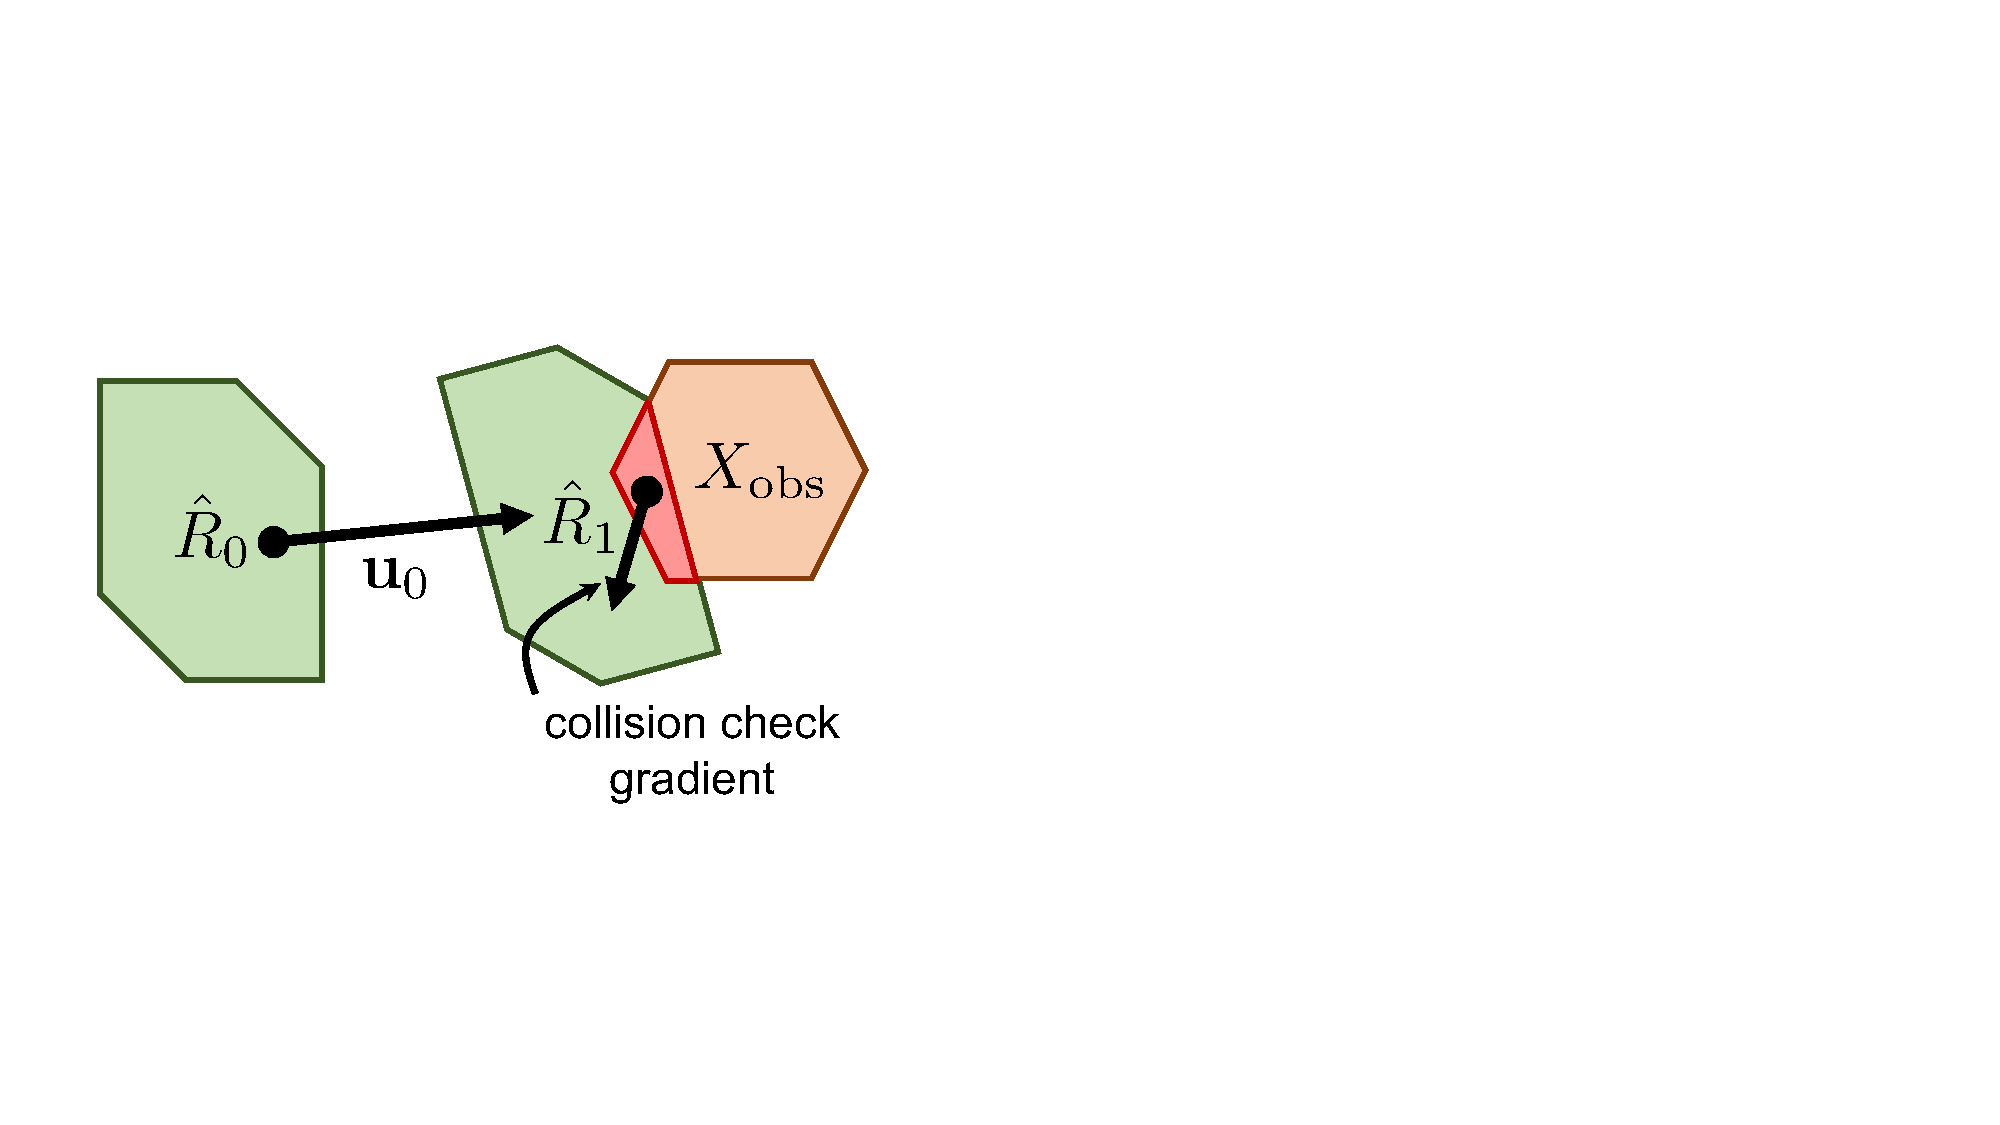
\includegraphics[scale=0.26]{Figures/collision_check_a.pdf}
%  \caption{}
%   \label{fig:Ng1} 
%\end{subfigure}
%\begin{subfigure}{0.49\columnwidth}
%\centering
%   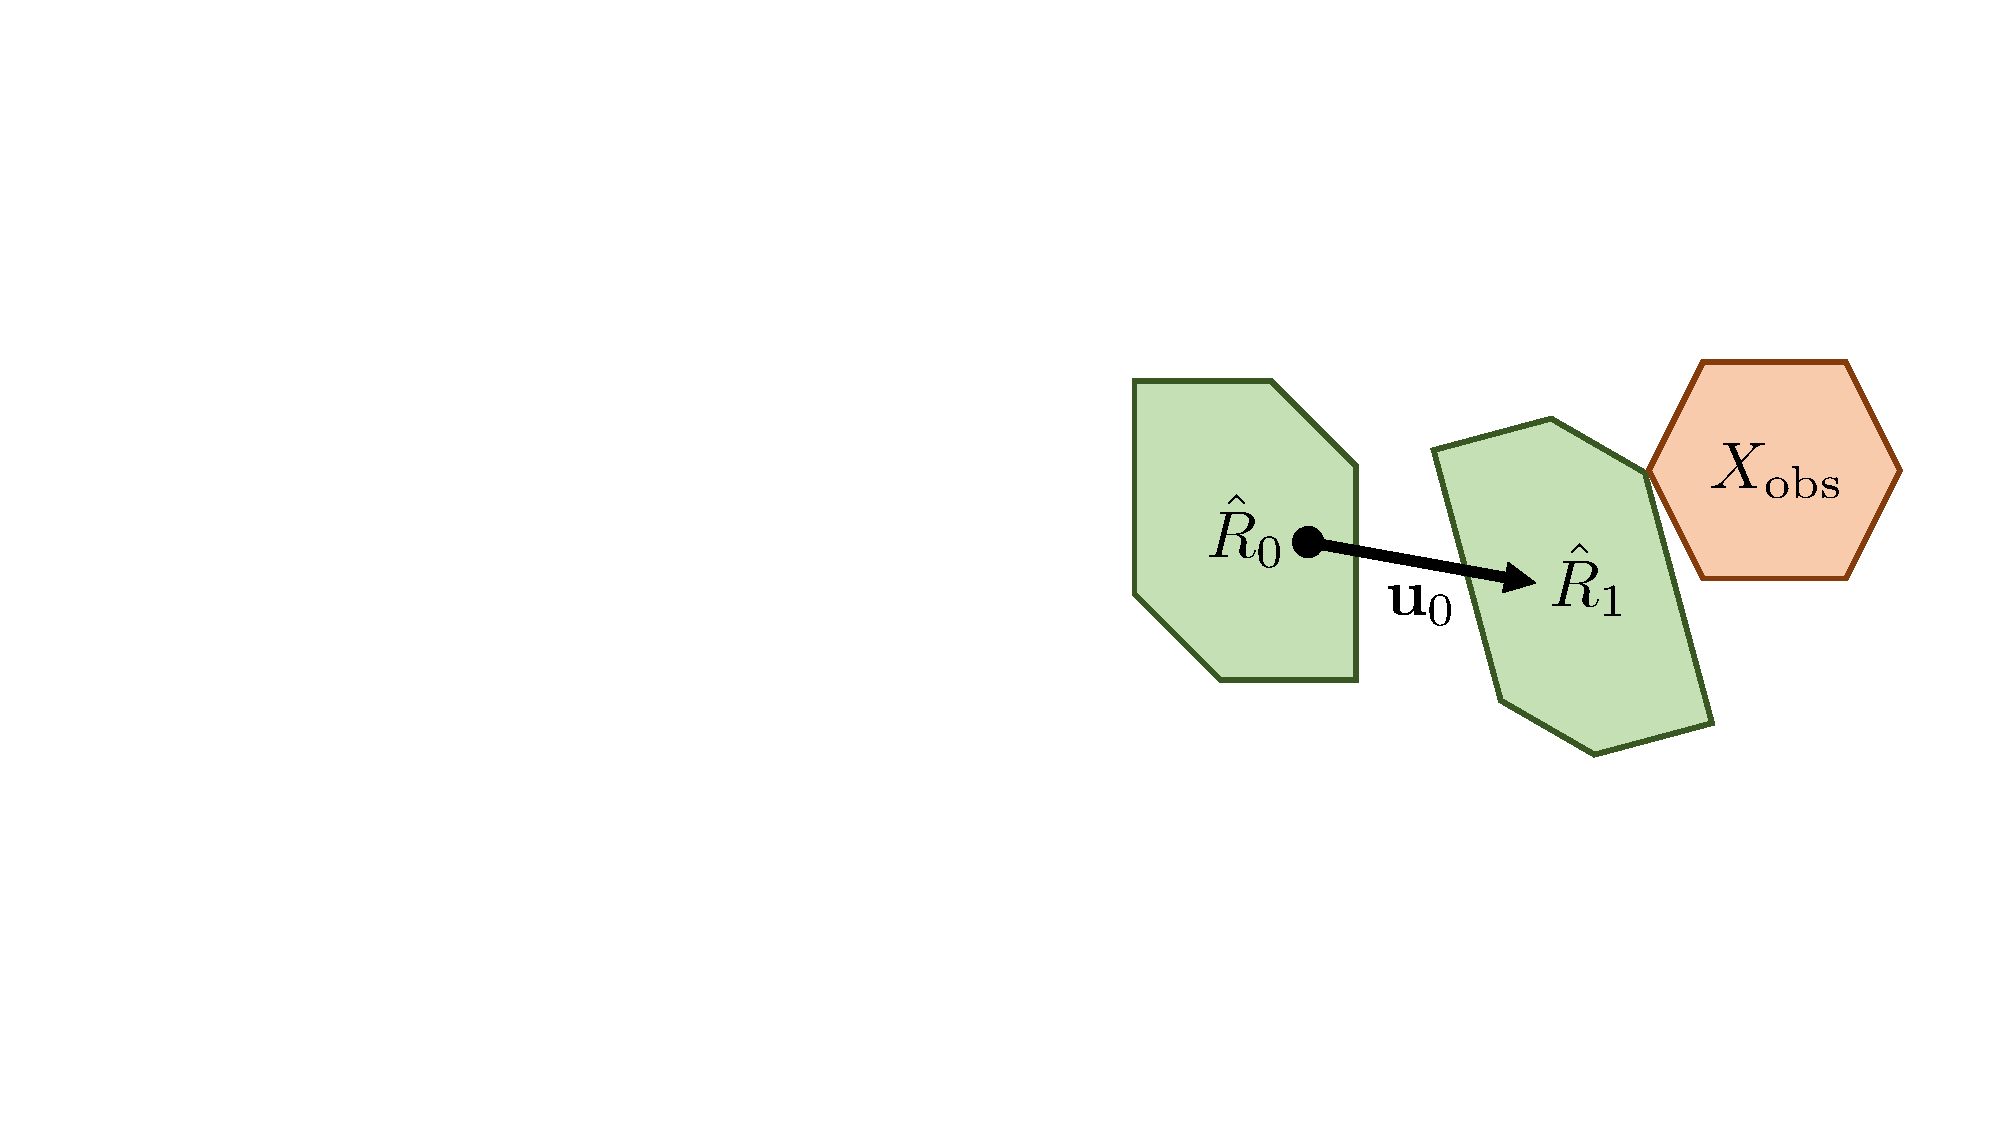
\includegraphics[scale=0.26]{Figures/collision_check_b.pdf}
%   \caption{}
%   \label{fig:Ng2}
%\end{subfigure}
%\caption{Our approach for pushing reachable sets, represented as zonotopes, out of intersection (see Alg. \ref{alg:adjust}).
%In (a), we compute the gradient of the collision check between the reachable set $\reachapprox_1$ and the obstacle $\statespace\obs$; in (b), we use constrained gradient descent to adjust $\action_0$ such that $\reachapprox_1\cap\statespace\obs = \emptyset$.}
%\label{fig:zonotope_intersection}
%\vspace{-2mm}
%\end{figure}

\begin{figure}
\centering     %%% not \center
\subfigure[]{\label{fig:Ng1}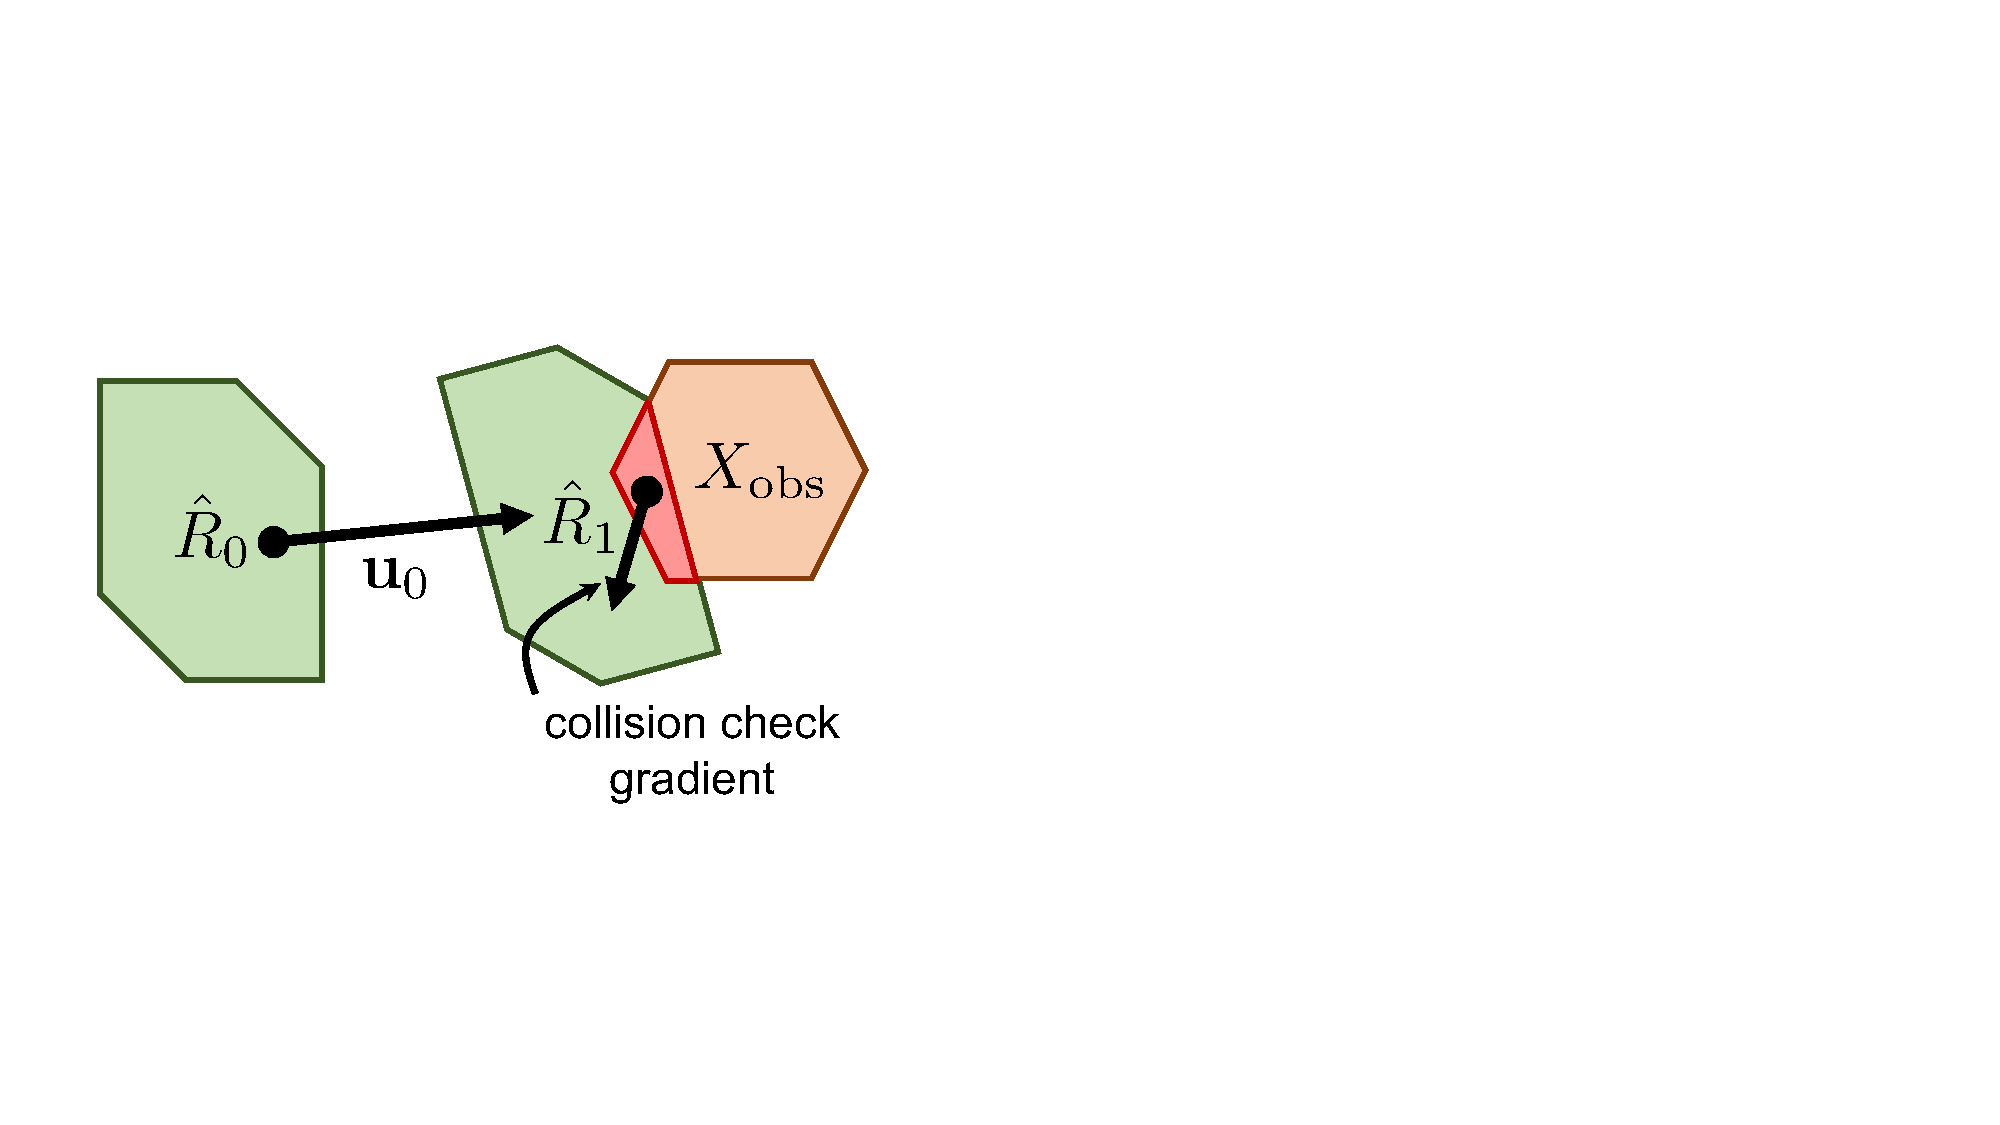
\includegraphics[width=0.4\columnwidth]{Figures/collision_check_a.pdf}}
\hspace{5mm}
\subfigure[]{\label{fig:Ng2}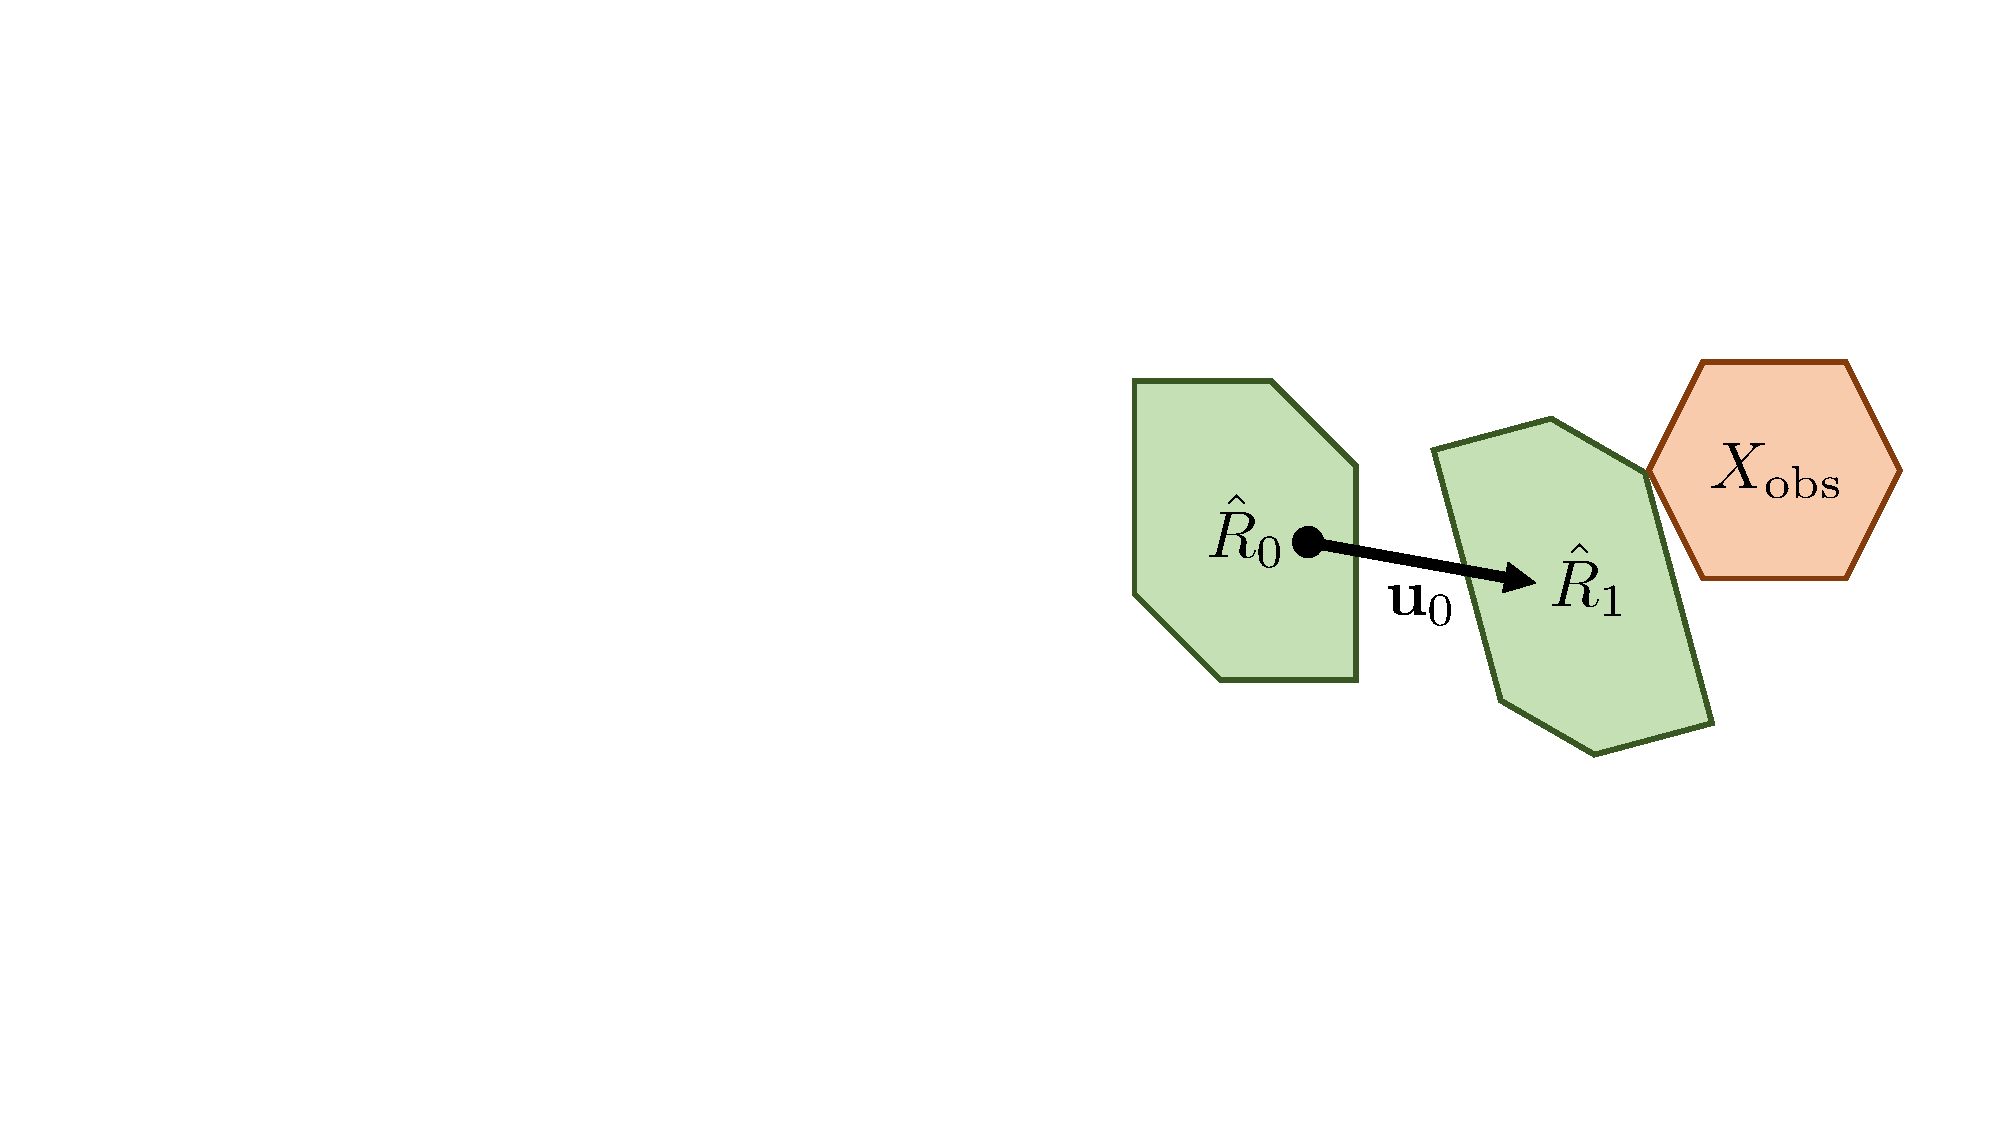
\includegraphics[width=0.4\columnwidth]{Figures/collision_check_b.pdf}}
\caption{We move zonotope reachable sets out of intersection (see Alg. \ref{alg:adjust}) by using the gradient of a collision check, shown in (a), to adjust $\action_0$ so the reachable sets are out of collision as shown in (b).} %between the reachable set $\reachapprox_1$ and the obstacle $\statespace\obs$; in (b), we use constrained gradient descent to adjust $\action_0$ such that $\reachapprox_1\cap\statespace\obs = \emptyset$.}
\label{fig:zonotope_intersection}
\vspace{-3mm}
\end{figure}


% \textbf{Differentiating the Collision Check.}~
We use gradient descent to move our reachable sets $\reachapprox_k$ out of collision.
Since we use \eqref{prog:collision_check} for collision checking, we differentiate its solution with respect to the problem parameters using \cite{amos2017optnet,chung2021constrained}.
Let $\hat{\ctr}_k$ denote the center of $\reachapprox_k$.
Per Algorithm \ref{alg:LipReachability}, $\reachapprox_k$ is a function of $\action_0,\cdots,\action_{k-1}$.
Let $(\coef\opt,v\opt)$ be an optimal solution to \eqref{prog:collision_check} when the problem parameters \tbold{(i.e., the input constrained zonotopes)} are $\reachapprox_k$ and an unsafe set.
Collision avoidance requires $v\opt > 1$ \cite[Prop. 2]{conf:const_zono}.
We compute the gradient $\nabla_{\RLaction_k} v\opt$ with respect to the input action (assuming a constant linearization point) using a chain rule recursion with $i = 0,\cdots,\nplan$ given by
\begin{align}\label{eq:collision_chain_rule}
    \nabla_{\RLaction_{h}} v\opt = \nabla_{\hat{\ctr}_k} v\opt
        \nabla_{\hat{\ctr}_{k - 1}} \hat{\ctr}_k
        \left(\prod_{j=h + 2}^{j = k - 1} \nabla_{\hat{\ctr}_{j - 1}} \hat{\ctr}_j\right) 
         \nabla_{\RLaction_{h}}  \hat{\ctr}_{h + 1},
\end{align}
with $h = k - i$.
The gradients of $\hat{\ctr}_k$ are given by
\begin{subequations}
\begin{align}
    &\nabla_{\hat{\ctr}_{k - 1}} \hat{\ctr}_k = (\vc{M}_{k - 1})_{(1:1+n),(1:1+n)},\ \regtext{and}
    \label{eq:collision_chain_rule_for_input_zono1} \\
    &\nabla_{u_{k - 1}} \hat{\ctr}_k = (\vc{M}_{k-1})_{:,(n+1:n+1+m)},
    \label{eq:collision_chain_rule_for_input_zono2}
\end{align}
\end{subequations}
where $\vc{M}_{k-1}$ is computed as in Algorithm \ref{alg:LipReachability}, Line \ref{ln:alglipMtilde}, and $n$ and $m$ are the state and action dimensions. 
After using  $\nabla_{\action_k}v\opt$ for gradient descent on $\action_k$, we project $\action_k$ to the set of feasible controls: $\proj_{\actionspace_k}(\action_k) = \argmin_{\vc{v} \in \actionspace_k} \left\{\norm{\action_k - \vc{v}}_2^2\right\}$.
The resulting controls may be unsafe, so we collision-check the final reachable sets at the end of Algorithm \ref{alg:adjust}.
% Using $\nabla_{\action_k}v\opt$ for gradient descent on $\action_k$ can cause ${\action_k \not\in U_k}$.
% Therefore, after each gradient step (Algorithm \ref{alg:adjust}, Line \ref{ln:adjust:get_gradient_and_step}), we project $\action_k$ into $\actionspace_k$ using a quadratic program: $\proj_{\actionspace_k}(\action_k) = \argmin_{\vc{v} \in \actionspace_k} \left\{\norm{\action_k - \vc{v}}_2^2\right\}$.
% Finding $\nabla_{\action_k}v\opt$ requires constrained gradient descent because we have constraints on the input actions.
% The problem in \eqref{eq:collision_chain_rule} can be solved either using projection or proximal operators since it is a convex optimization problem.

\begin{algorithm}[t]
\caption{Adjusting Unsafe Actions}
\label{alg:adjust}

\KwInput{plan $\plan_k = (\action_j)_{j=k}^{\nplan}$, obstacles $\statespace\obs$, initial reachable set $\reachapprox_k$, step size $\gamma$, time limit $t\lbl{max}$, time steps required to stop $n\brk$} 
// note $\plan_k$ has failsafe $\action\brk$ for all $j > k+\nplan$

$\plan\safe \leftarrow \plan_k$ // initialize with given plan

\For{$j = k:(k+\nplan + n\brk)$\label{ln:adjust:for_loop}}{
    \While{time limit not exceeded\label{ln:adjust:while_loop}}{
        $(\reachapprox_j)_{j=k}^{k+\nplan} \leftarrow \reachfunc{\reachapprox_j,\plan\safe}$ // use Alg. \ref{alg:LipReachability} \label{ln:adjust:reach}
    
        $v\opt \leftarrow $ collision check $\reachapprox_j \cap \statespace\obs$ using \eqref{prog:collision_check} \label{ln:adjust:collision_check}
        
        \uIf{$v\opt \leq 1$ (i.e., in collision)}{        
            $\action_j \leftarrow \proj_{\actionspace_j}\left(\action_j + \gamma \nabla_{\action_j} v\opt\right)$ // using \eqref{eq:collision_chain_rule} \label{ln:adjust:get_gradient_and_step}
            
            %$\action_j \leftarrow \proj_{\actionspace_j}(\action_j)$ \label{ln:adjust:project}
            
            %$\plan\safe\idx{j} \leftarrow \action_j$ // update current action \label{ln:adjust:update_action}
        }
        % \uElseIf{$\vcstate_n$ is not stopped}{
        %     $\action_j \leftarrow \tfrac{n-j}{n}\action_j + \tfrac{j}{n}\action\brk$ // add failsafe \label{ln:adjust:add_failsafe}
        % }
        \Else{
            \textbf{break} and restart inner while loop \label{ln:adjust:break_while_loop}
        }
    }
}

\eIf{all $\reachapprox_j \cap \statespace\obs = \emptyset$ and $\vcstate_n$ is stopped\label{ln:adjust:check_if_safe}}{
    % $p \leftarrow \sum_{k=0}^n \norm{\plan\idx{k} - \plan\safe\idx{k}}_2$ // compute penalty
    
    \textbf{return} $\plan\safe = (\action_j)_{j=k}^{\nplan}$ // found new safe plan% and $p$
}{
    \textbf{return} error ``unsafe'' // failed to find safe plan\label{ln:adjust:return_unsafe}
}
\end{algorithm}



\begin{figure*}[t]
\centering     %%% not \center
\begin{subfigure}[h][\tbold{Turtlebot3 Environment}]{\label{fig:tb_env}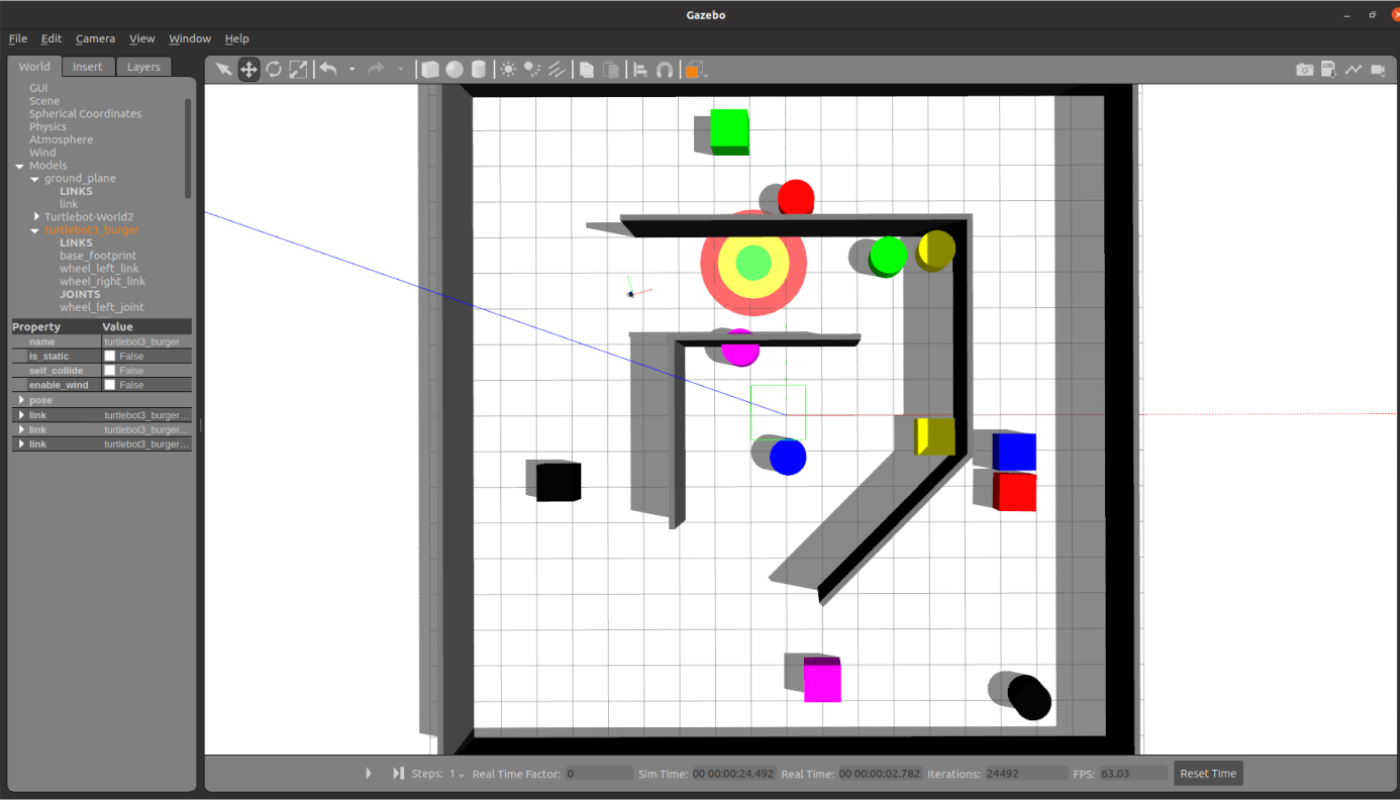
\includegraphics[scale=0.1]{Figures/Turtlebot-Env.png}}
\end{subfigure}
\begin{subfigure}[h][\tbold{Quadrotor Environment}]{\label{fig:quad_env}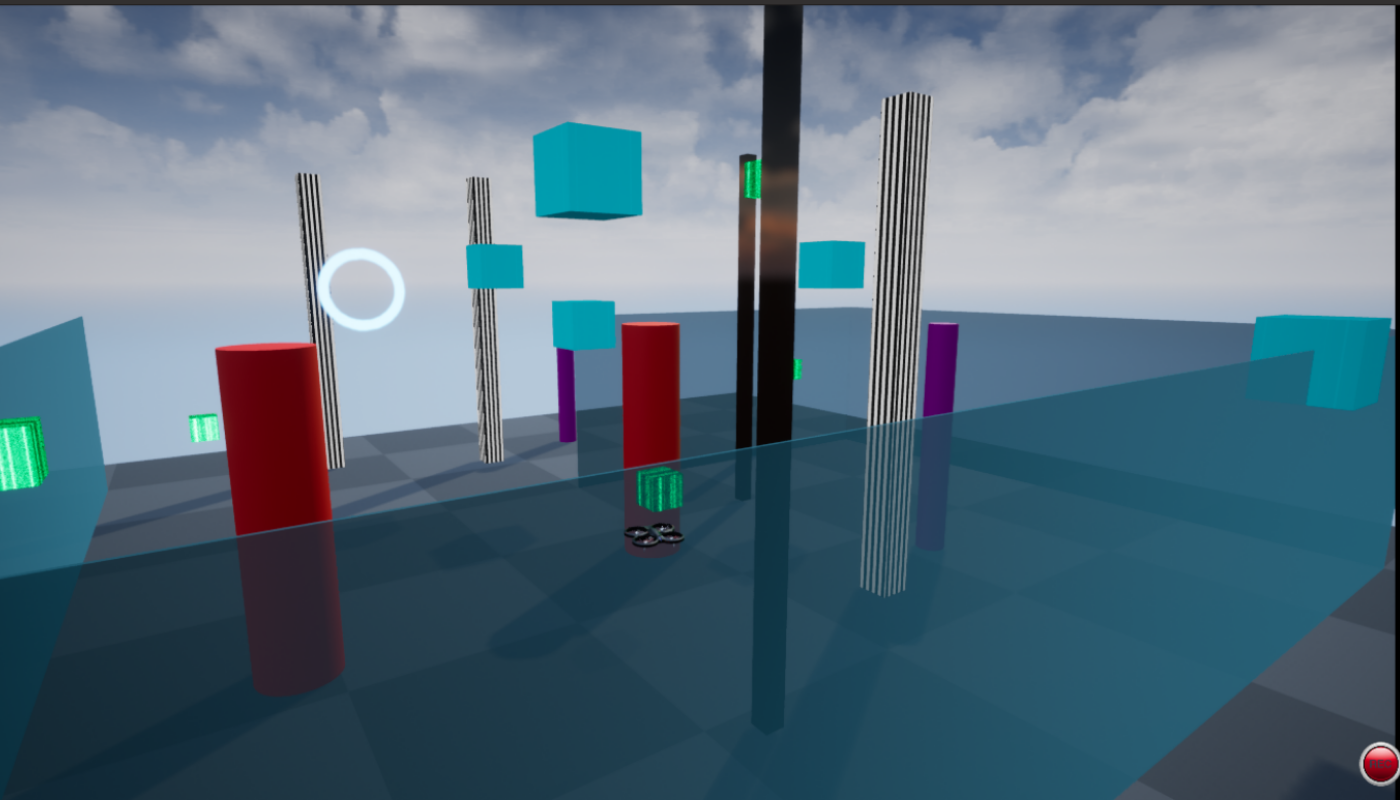
\includegraphics[scale=0.1]{Figures/Quadrotor-Env.png}}
\end{subfigure}
\begin{subfigure}[h][\tbold{Hexarotor Environment}]{\label{fig:hex_env}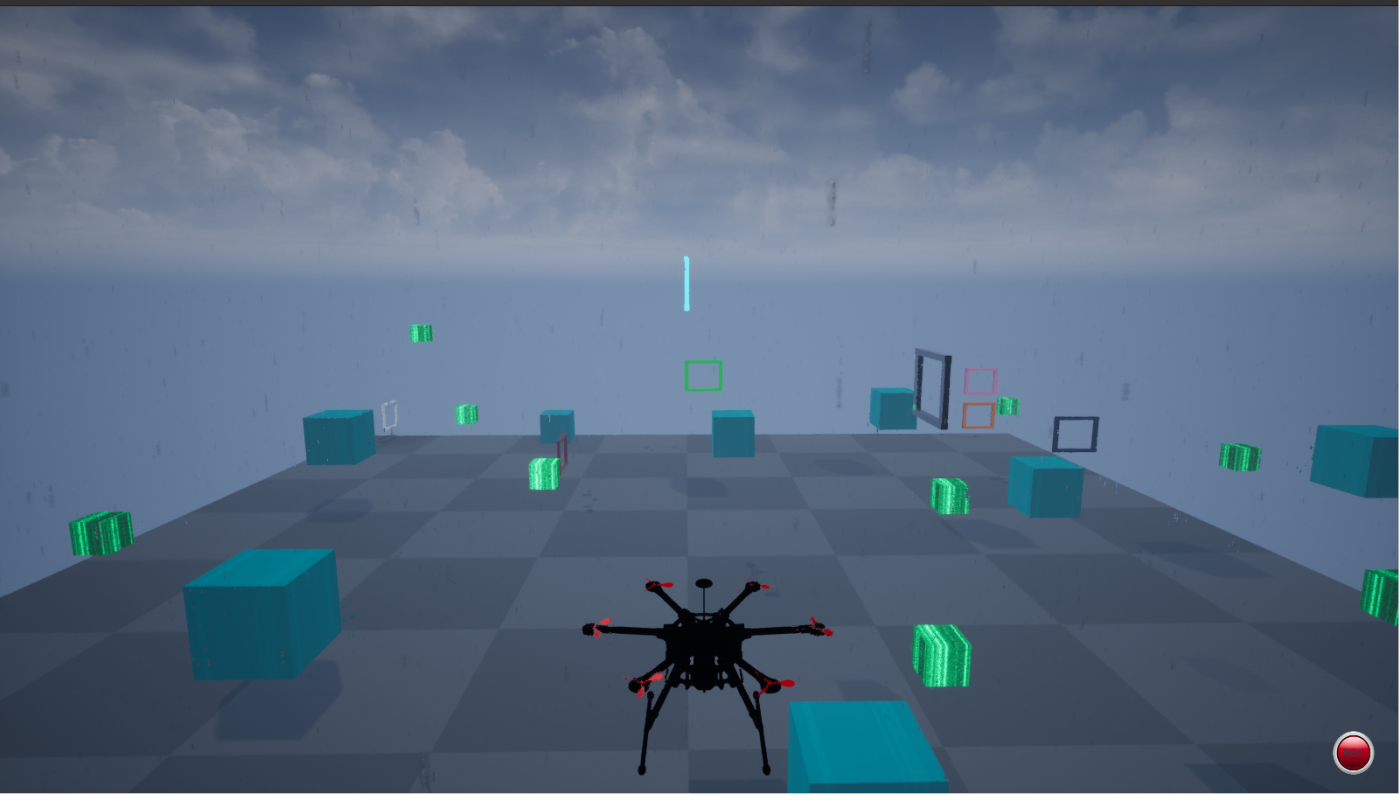
\includegraphics[scale=0.1]{Figures/Hexarotor-Env.png}}
\end{subfigure}
%\hspace{10mm}
%\subfigure[Arrival and collisions rates are in bold and dashed lines, respectively.]{\label{fig:Ng2}\includegraphics[scale=0.25]{Figures/turtlebot_safety.png}}
\caption{\tbold{Evaluation Environments.}}
\label{fig:sim_envs}
\vspace{-5mm}
\end{figure*}

 \subsection{Analyzing Safety}
%\textbf{Analyzing Safety.}
We conclude this section by formalizing the notion that BRSL enables safe RL.

\begin{theorem}\label{thm:BRSL_is_safe}
Suppose the assumptions on the robot and environment from Section \ref{sec:pb} all hold, and, at time $k = 0$, the robot is \tbold{at safe state}.
Suppose also that, at each time $k > 0$, the robot \tbold{rolls out} a new $\plan_k$, then adjusts the plan using Algorithm \ref{alg:adjust}.
Then, the robot is guaranteed to be safe at all times $k \geq 0$.
\end{theorem}
\begin{proof}
We prove the claim by induction on $k$.
At time $0$, the robot can apply $\action\brk$ to stay safe for all time.
Assume a safe plan exists at time $k \in \N$.
Then, if the output of Algorithm \ref{alg:adjust} is unsafe (no new plan found), the robot can continue its previous safe plan; otherwise, if a new plan is found, the plan is safe for three reasons.
First, the black-box reachability in Algorithm \ref{alg:LipReachability} is guaranteed to contain the true reachable set of the system \cite[Theorem 2]{alanwar2020data_conf}, because process noise is bounded by a zonotope as in Assumption \ref{assumption:noise_zonotope}.
Second, when adjusting an unsafe plan with Algorithm \ref{alg:adjust}, the zonotope collision check is guaranteed to always detect collisions \cite[Prop. 2]{conf:const_zono} to assess if $\reachapprox_j \cap \statespace\obs$ is empty for each time step $j$ of the plan.
Third, Algorithm \ref{alg:adjust} requires that, after $\nplan$ timesteps, the robot is stopped, so the new plan contains a failsafe manuever, and the robot can safely apply $\action\brk$ for all time $j \geq k+\nplan$.
\end{proof}



% \tbold{We note that the accuracy of the environment model, trained online, does not affect the above result.
% This is because we enforce safety via data-driven reachability; so, Theorem \ref{thm:BRSL_is_safe} will hold as long as the data (collected before runtime) are still representative of the robot's dynamics at runtime.
% We leave updating the data online for future work.}
We note that the accuracy of the environment model, trained online, does not affect safety; Theorem \ref{thm:BRSL_is_safe} holds as long as the offline data are representative of the robot's dynamics at runtime.
We leave updating the data online for future work.

% Next, we evaluate BRSL numerically.